\documentclass[11pt]{beamer}
\usetheme{EastLansing}
\usecolortheme{default}
\usepackage[utf8]{inputenc}
\usepackage{amsmath, amssymb, amsfonts, amsthm, mathtools}
\usepackage{tikz,tikz-cd}
\usepackage{graphicx}
\graphicspath{ {./images/} }
\usepackage{biblatex}
\author[K. Sreeman Reddy]{\href{http://iamsreeman.github.io/}{\textbf{Kasi Reddy Sreeman Reddy}}\linebreak\text{2nd year physics student}\linebreak\text{\href{http://iamsreeman.github.io/MA109}{http://iamsreeman.github.io/MA109}}}
\title{MA 109 Tutorial 3}
%\setbeamercovered{transparent} 
%\setbeamertemplate{navigation symbols}{} 
\logo{
\includegraphics[width=.1\textwidth]{logo}} 
\institute[]{IIT Bombay} 
\date{09-Dec-2020}
%\subject{}
\BeforeBeginEnvironment{definition}{
    \setbeamercolor{block title}{use=example text,fg=white,bg=example text.fg!75!black}
    \setbeamercolor{block body}{parent=normal text,use=block title example,bg=block title example.bg!10!bg}
}
\AfterEndEnvironment{definition}{
        \setbeamercolor{block title}{use=structure,fg=white,bg=structure.fg!75!black}
        \setbeamercolor{block body}{parent=normal text,use=block title,bg=block title.bg!10!bg}
}
\BeforeBeginEnvironment{theorem}{
    \setbeamercolor{block title}{use=example text,fg=white,bg=example text.fg!75!black}
    \setbeamercolor{block body}{parent=normal text,use=block title example,bg=block title example.bg!10!bg}
}
\AfterEndEnvironment{theorem}{
        \setbeamercolor{block title}{use=structure,fg=white,bg=structure.fg!75!black}
        \setbeamercolor{block body}{parent=normal text,use=block title,bg=block title.bg!10!bg}
}
%---------------------------------------------------------
\begin{document}
\begin{frame}
\titlepage
\end{frame}
%---------------------------------------------------------


\section{Sheet 2}
\begin{frame}
\frametitle{Q)8}
(ii) Let $f'(x)=x+1$. It satisfies all the given conditions. So, $f(x)=\frac{x^2}{2}+x+c$ satisfies.\\
(iii) Apply MVT(Mean Value Theorem) for $f'(x)$ on $[0,x]$ for some $x>0$
\begin{align*}
\dfrac{f'(x)-f'(0)}{x-0}&=f''(c_1)\geq 0\\
\Rightarrow f'(x)&\geq 1
\end{align*}
Similarly doing for $f(x)$
\begin{align*}
\dfrac{f(x)-f(0)}{x-0}&=f'(c_2)\geq 1\\
\Rightarrow f(x)&\geq f(0)+x\\
\Rightarrow f(100-f(0))&\geq 100\\
\Rightarrow \forall x >100-f(0), f(x)>100
\end{align*}
So no such function exists.
\end{frame}
\begin{frame}
\frametitle{Q)8}
(iv) $f(x)=e^x$ satisfies all the conditions needed. You can find other solutions also. $g(x)=\dfrac{x+e^x}{2}$ also satisfies all the conditions needed. Here $g'(x)=\frac{1+e^x}{2}$, $g''(x)=\frac{e^x}{2}$
\end{frame}
\begin{frame}
\frametitle{Q)10(i)}
\begin{align*}
f(x)&=2x^{3}+2x^{2}-2x-1\\
f'(x)&=6x^{2}+4x-2x=2(x+1)(3x-1)\\
f''(x)&=12x+4
\end{align*}
Observe that $f'(x)>0$ in $(-\infty,-1)\cup (\frac{1}{3},\infty)$, $f'(x)<0$ in $(-1,\frac{1}{3})$ and $f'(-1)=f'(\frac{1}{3})=0$. So $f(x)$ has a local maximum at $x = -1$; and a local minimum at $x =\frac{1}{3}$. Also observe that $f''(x) = 12x + 4>0$ in $(-\frac{1}{3},\infty)$, <0 in $(-\infty,-\frac{1}{3}$ and $f''(-\frac{1}{3})=0$ so $x=-\frac{1}{3}$ is a point of inflection. This function also doesn't have any asymptotes.
\end{frame}
\begin{frame}
\frametitle{Q)10(i)}
\begin{figure}[t]
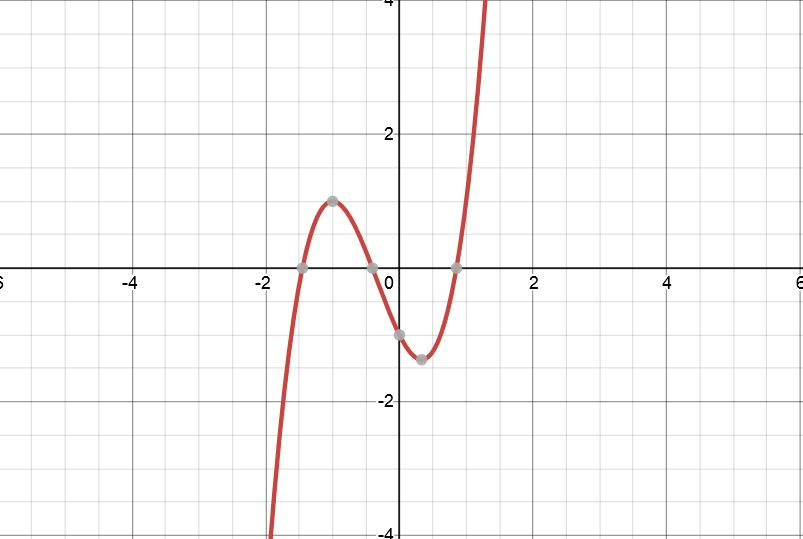
\includegraphics[scale=0.5]{graph}
\centering
\end{figure}
\end{frame}
\begin{frame}
\frametitle{Q)11}
\begin{figure}[t]
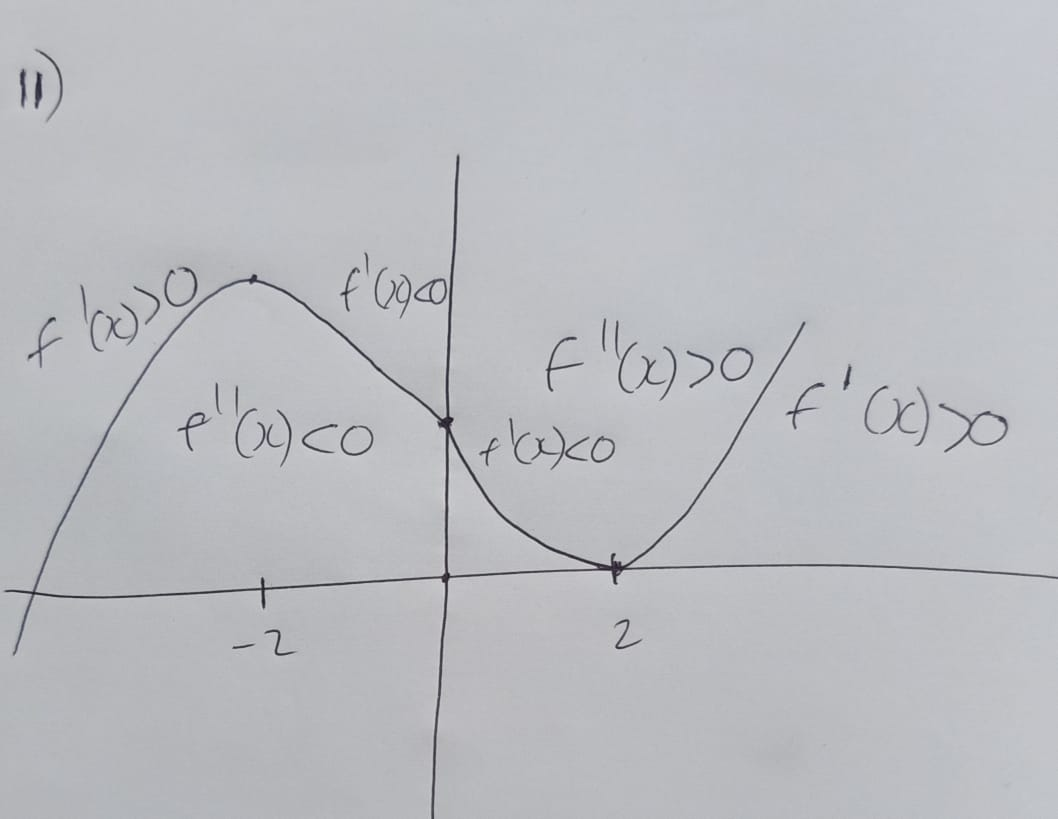
\includegraphics[scale=0.2]{11}
\centering
\end{figure}
Also $f(x)=\frac{3}{4}(\frac{x^3}{3}-4x)+4$ is a possible solution. Draw it.
\end{frame}
\section{Sheet 3}
\begin{frame}
\frametitle{Q)1(ii)}
Here $f(x)=arctan(x)$. From Taylor's theorem we can write that
$$f(x)=\sum_{r=0}^{n}\dfrac{f^{(r)(x_0)}}{r!}(x-x_0)^{r}+\dfrac{f^{(n+1)}(c_x)}{(n+1)!}(x-x_0)^{n+1}$$
where $c_x\in (x_0,x) or \in (x,x_0)$. Here I wrote $c_x$ because it depends on $x$. $f^{(1)}(x)=\frac{1}{1+x^2}$, from there you can go on differentiating and get all derivatives. But to express them as $x$ and $n$ is not easy. But using the complex number $i$ we can simply write is as
\begin{align*}
f^{n}(x)=\frac{1}{2}(i(-1)^{n}(n-1)!)((x-i)^{-n}-(x+i)^{-n})
\end{align*}
This form can be obtained by using $\frac{1}{1+x^2}=\frac{1}{2i}(\frac{1}{x-i}-\frac{1}{x+i})$ and differentiating. Although since this course considers only $\mathbb{R}$ the induction method is better.
\end{frame}
\begin{frame}
We can also do this using integration also like $f'=\frac{1}{1+x^2}$ express it as a geometric series and integrate term by term. But why we can integrate term by term is beyond the syllabus of this course. It will be taught in a MA 403 topic called sequences and series of functions. If you are interested read about \href{https://en.wikipedia.org/wiki/Uniform_convergence}{Uniform convergence}. \textbf{But for this course you can integrate the series without justification.} Here $x_0=0$, so
$$R_n(x)=\frac{f^{(n+1)}(c_x)(x-0)^{n+1}}{(n+1)!}$$
\end{frame}
\begin{frame}

\frametitle{Q)2}
You can write the function as $f(x)=(x-1)^3$. Clearly it is the Taylor series. You can also find derivatives and do. For any polynomial the Taylor series is exactly the polynomial itself.
\end{frame}
\begin{frame}
\frametitle{Q)4}
Let us denote the partial sums of of the given series by $s_m(x)$. We would like to show that $|s_m(x) - s_n(x)|$ can be made arbitrarily small whenever m and n are sufficiently large. Without loss of generality assume that $m>n$. We see that
$$|s_m(x) -s_n(x)|=|\sum_{k=n+1}^{m}\frac{x^k}{k!}|\leq |\frac{x^n}{n!}|\left(\frac{1}{2}+\frac{1}{4}\cdots +\frac{1}{2^{m-n}}\right)\leq 2\frac{|x^2|}{n!}$$.

If $N$ is made sufficiently large and $n > N$, the last expression can be made as small as we please.
\end{frame}
\begin{frame}
\frametitle{Q)5}
The taylor series for $e^x=\sum_{r=0}^{\infty}\frac{x^n}{n!}$. So,
\begin{align*}
\frac{e^x}{x}&= \sum_{r=0}^{\infty}\frac{x^{n-1}}{n!}\\
\int_{a}^{b} \frac{e^x}{x}dx&=\int_{a}^{b} \left( \sum_{r=0}^{\infty}\frac{x^{n-1}}{n!}dx\right)\\
\int_{a}^{b} \frac{e^x}{x}dx&=\sum_{r=0}^{\infty}\left(\int_{a}^{b} \frac{x^{n-1}}{n!}dx\right)\\
\int \frac{e^x}{x}dx&=\sum_{r=0}^{\infty}\left(\int\frac{x^{n-1}}{n!}dx\right)\\
\int \frac{e^x}{x}dx&=\sum_{r=0}^{\infty}\left(\int\frac{x^{n}}{(n)n!}dx\right)+c
\end{align*}
Here the interchange of $\sum$ and $\int$ are assumed.
\end{frame}
\end{document}